\documentclass[12pt, a4paper]{article} 
\usepackage{here}
\usepackage{enumerate}
\usepackage{latexsym}
\usepackage{amsmath,amssymb}
\usepackage{graphicx}
\usepackage[demo]{graphicx}
\usepackage{subfig}
\usepackage[outdir=./]{epstopdf}
\DeclareGraphicsExtensions{.eps}
\usepackage{bm}
\usepackage{geometry}
\usepackage{listings}
\usepackage{color} %red, green, blue, yellow, cyan, magenta, black, white
\linespread{1.5}
\definecolor{mygreen}{RGB}{28,172,0} % color values Red, Green, Blue
\definecolor{mylilas}{RGB}{170,55,241}
\lstset{language=Matlab,%
	%basicstyle=\color{red},
	breaklines=true,%
	morekeywords={matlab2tikz},
	keywordstyle=\color{blue},%
	morekeywords=[2]{1}, keywordstyle=[2]{\color{black}},
	identifierstyle=\color{black},%
	stringstyle=\color{mylilas},
	commentstyle=\color{mygreen},%
	showstringspaces=false,%without this there will be a symbol in the places where there is a space
	% numbers=left,%
	numberstyle={\tiny \color{black}},% size of the numbers
	numbersep=9pt, % this defines how far the numbers are from the text
	emph=[1]{for,end,break},emphstyle=[1]\color{red}, %some words to emphasise
	%emph=[2]{word1,word2}, emphstyle=[2]{style},    
}
%\usepackage{amsmath,amsfonts,amssymb} 

\geometry{left = 1cm, right=1cm, top= 1cm, bottom=2cm}
\title{MAE5403 (Linear System Control Design Problem) \textbf {Unmanned Helicopter Controller Design} }


\author{\textbf {Linzhu Yue 1155144991}}
\begin{document} 
\maketitle
\begin{enumerate}[1.]\setlength{\itemsep}{1cm}

%Abstract%	
\item  \textbf{Abstract}


\hspace{0.5em}In this Unmanned Helicopter case. We consider 9 state space variable. There are three angle(Roll,Pitch,Yaw),three angular rates and three unmeasured
variable($a_s,b_s,\delta_{ped,int}$). This system also has three inputs and three dsiturbance wind noise$\delta_{lat},\delta_{lon},\delta_{ped}$ and $u_{wind},u_{wind},\delta_{wind}$,respectively.
I choose LQG technique in this case for Inner-loop Flight control. I also try $H_{\infty}$,but I have some problem about reduced order Controller design,
I can not caculate the right nums. So I decide to use LQG for this case. And I use simulink to simulation my controller,It have good performance that I will show in Part2(Results analysis).

\item  \textbf{ Part1: Mathmactics and Fligh dynamics model analysis}
\begin{enumerate}[(a)]
	\item 
        Here,We Let 
        \begin{align*}
            \dot{x} = Ax+Bu+Ew\\
            y=C_1x+D_1v
        \end{align*} And the noise \textbf{v} is the measurement output noise,In this case i choose the white noise for output measurement noise.
        The state variable is  
        $x=\begin{Bmatrix}
            \phi  \\
            \theta \\
            p       \\
            q \\
            a_s \\
            b_s \\
            r \\
            \delta_{ped,int} \\
            \psi
            \end{Bmatrix}
        $;
        $u=\begin{Bmatrix}

            \delta_{lat} \\
            \delta_{lon} \\
            \delta_{ped} 
            \end{Bmatrix}
        $;
        $w=\begin{Bmatrix}

            u_{wind} \\
            v_{wind} \\
            w_{wind} 
            \end{Bmatrix}
        $;
    \item And from dynamics linearization model,we also obtain the A,B and E martix,They showed the fellowing. \\
        $A=\begin{bmatrix}
            0& 0& 1      &       0&        0&        0&   0.0009&       0& 0 \\
            0& 0& 0      &  0.9992&        0&        0&  -0.0389&       0& 0 \\
            0& 0& -0.0302& -0.0056&  -0.0003& 585.1165&  11.4448& -59.529& 0 \\
            0& 0& 0      & -0.0707& 267.7499&  -0.0003&        0&       0& 0 \\
            0& 0& 0      & -1.0000&  -3.3607&   2.2223&        0&       0& 0 \\
            0& 0& -1     &       0&   2.4483&  -3.3607&        0&       0& 0 \\
            0& 0& 0.0579 &  0.0108&   0.0049&   0.0037& -21.9557&   114.2& 0 \\
            0& 0& 0      &       0&        0&        0&       -1&       0& 0 \\
            0& 0& 0      &  0.0389&        0&        0&   0.9992&       0& 0 \\

            \end{bmatrix}
        $; \\
        $B=\begin{bmatrix}
            0      &0        &0 \\
            0      &0        &0 \\
            0      &0        &43.3635 \\
            0      &0        &0 \\
            0.2026 &2.5878   &0 \\
            2.5878 &-0.0663  &0 \\
            0      &0        &-83.1883 \\
            0      &0        &-3.8500 \\
            0      &0        &0 

            \end{bmatrix}
        $;
        $E=\begin{bmatrix}
            0       &0      &      0 \\
            0       &0      &      0 \\
            -0.0001 &0.1756 &-0.0395 \\
            0.0000  &0.0003 & 0.0338 \\
            0       &0      &      0 \\
            0       &0      &      0 \\
            -0.0002 &-0.3396& 0.6424 \\
            0       &0      &      0 \\
            0       &0      &      0 
            \end{bmatrix}
        $;\\

        $C_1=\begin{bmatrix}
            1 &0 &0 &0 &0 &0 &0 &0 &0 \\
            0 &1 &0 &0 &0 &0 &0 &0 &0 \\
            0 &0 &1 &0 &0 &0 &0 &0 &0 \\
            0 &0 &0 &1 &0 &0 &0 &0 &0 \\
            0 &0 &0 &0 &0 &0 &0 &0 &0 \\
            0 &0 &0 &0 &0 &0 &0 &0 &0 \\
            0 &0 &0 &0 &0 &0 &1 &0 &0 \\
            0 &0 &0 &0 &0 &0 &0 &0 &0 \\
            0 &0 &0 &0 &0 &0 &0 &0 &1 
            \end{bmatrix}
        $;

    \item Choose the LQG technique for this case. Before we start the design, we need to know the pair (A,B) and (A,C1)is controllable and observable.
        It's obvious full rank with the matlab command rank(ctrb(A,B)) and rank(obsv(A,C1)). So we can do the job now.
        we need to three steps for solving this case, I will show as fellowing:\\
        \textbf{First:},We need to design a LQR control law $ u=-Fx$,and we need to choose the Matirx Q and R($ Q\geq 0$,$ R \geq 0$).
        Here is the  Q and R matrix in my simulation:\\
        $Q=\begin{bmatrix}
            1&     0&     0&     0&     0&     0&     0&     0&     0 \\
            0&     1&     0&     0&     0&     0&     0&     0&     0 \\
            0&     0&     1&     0&     0&     0&     0&     0&     0 \\
            0&     0&     0&     1&     0&     0&     0&     0&     0 \\
            0&     0&     0&     0&     0&     0&     0&     0&     0 \\
            0&     0&     0&     0&     0&     0&     0&     0&     0 \\
            0&     0&     0&     0&     0&     0&     1&     0&     0 \\
            0&     0&     0&     0&     0&     0&     0&     0&     0 \\
            0&     0&     0&     0&     0&     0&     0&     0&     1 
            \end{bmatrix}
        $;$ R =0.001$ \\
        Then,use Matlab function icare(\textbf{Note:}are function can not solve B nonsymmetric,so i choose icare more general function) to solve the Riccati Equtaion $ PA+A^TP-PBR^{-1}B^TP+Q=0 $, $ P \geq 0 $,$ F=R^{-1}B^TP $;
        The matlab code is:
        \begin{lstlisting}
            [X1,K1,L1] = icare(A,[],Q'*Q,[],[],[],-B*B');
            F=inv(R)*B'*X1;
            Abk=A-B*F;
            eigabk=eig(Abk);
        \end{lstlisting} 
        Then,We obtain the gain F matrix as fellow: \\
        \\
        $F=1.0e+04 *\begin{bmatrix}
            0.0943&    0.0035&    0.0652&    0.0039&    0.1251&    1.5944&    0.0356&   -0.0087&    0.0332 \\
           -0.0046&    0.0999&   -0.0025&    0.0724&    1.0974&   -0.0017&   -0.0012&    0.0003&    0.0028 \\
            0.0331&    0.0042&    0.0354&    0.0004&   -0.0045&   -0.0391&   -0.0721&   -0.1079&   -0.0943 
            \end{bmatrix}
        $; \\
        And the matrix $ A-BF$ is show: \\
        \\
        $Abk=1.0e+04 *\begin{bmatrix}
            \begin{smallmatrix}
            0&         0&    0.0001&         0&         0&         0&    0.0000&         0&         0 \\
            0&         0&         0&    0.0001&         0&         0&   -0.0000&         0&         0 \\
      -1.4344&   -0.1806&   -1.5341&   -0.0177&    0.1934&    1.7547&    3.1298&    4.6733&    4.0883 \\
            0&         0&         0&   -0.0000&    0.0268&   -0.0000&         0&         0&         0 \\
      -0.0071&   -0.2591&   -0.0067&   -0.1883&   -2.8654&   -0.3184&   -0.0041&    0.0010&   -0.0139 \\
      -0.2442&   -0.0023&   -0.1689&   -0.0053&   -0.2506&   -4.1263&   -0.0922&    0.0225&   -0.0858 \\
       2.7517&    0.3465&    2.9430&    0.0339&   -0.3711&   -3.2539&   -6.0041&   -8.9653&   -7.8429 \\
       0.1273&    0.0160&    0.1362&    0.0016&   -0.0172&   -0.1506&   -0.2779&   -0.4154&   -0.3630 \\
            0&         0&         0&    0.0000&         0&         0&    0.0001&         0&         0 
        \end{smallmatrix}    
        \end{bmatrix}
        $; \\
        \\
        And the eigvalues is show:\\
        \\
        $Eigvalues=1.0e+04 *\begin{bmatrix}
            -7.9558 + 0.0000i \\ 
            -4.1816 + 0.0000i \\
            -2.8032 + 0.0000i \\
            -0.0023 + 0.0000i \\
            -0.0016 + 0.0000i \\
            -0.0005 + 0.0000i \\
            -0.0001 + 0.0000i \\
            -0.0001 - 0.0000i \\
            -0.0001 + 0.0000i
            \end{bmatrix}
        $; We can see all eigvalue have negative real part.\\
        \textbf{Second:},We need to use Kalman filter for the plant,
        $ \dot{\hat{x}}=A\hat{x}+K_e(y-\hat{y}),\hat{y}=C_1\hat{x}$. \\
        We also use icare to sove Riccati Equtaion:\\
        $ P_eA^T+AP_e-P_eC^TR_e^{-1}CP_e+Q_e=0 $, $ P_e \geq 0 $,$ Ke=P_eC^TR_e^-1 $ \\
        And here we choose the $ Q_e $ and $ R_e $ matrix as fellowing:\\
        $Q_e=1.0e-03 *\begin{bmatrix}
            1.0000&         0&         0&         0&         0&         0&         0&         0&         0 \\
                 0&    1.0000&         0&         0&         0&         0&         0&         0&         0 \\
                 0&         0&    1.0000&         0&         0&         0&         0&         0&         0 \\
                 0&         0&         0&    1.0000&         0&         0&         0&         0&         0 \\
                 0&         0&         0&         0&    1.0000&         0&         0&         0&         0 \\
                 0&         0&         0&         0&         0&    1.0000&         0&         0&         0 \\
                 0&         0&         0&         0&         0&         0&    1.0000&         0&         0 \\
                 0&         0&         0&         0&         0&         0&         0&    1.0000&         0 \\
                 0&         0&         0&         0&         0&         0&         0&         0&    1.0000 
            \end{bmatrix}
        $;\\
        $ R_e=0.004 $ \\
        Using Matlab code as fellow:\\
        \begin{lstlisting}
            [X2,K2,L2] = icare(A,[],Qe'*Qe,[],[],[],-C1*C1');
            % Pk=are(A,C1,Qe)
            Ke=X2*C1'*inv(Re)
            Ack=A-Ke*C1
            eigack=eig(Ack)
        \end{lstlisting} 
        And we obtain Ke and $Ack=A-K_eC_1$ and Ack eigenvalues:
        Then,We obtain the F matrix as fellow: \\
        $K_e=\begin{bmatrix}
            0.2500&    0.0000&    0.0014&   -0.0023&         0&         0&    0.0007&         0&    0.0000 \\
            0.0000&    0.2500&   -0.0009&    0.0031&         0&         0&   -0.0005&         0&   -0.0000 \\
            0.0014&   -0.0009&    0.0001&   -0.0000&         0&         0&    0.0000&         0&   -0.0000 \\
           -0.0023&    0.0031&   -0.0000&    0.0001&         0&         0&   -0.0000&         0&    0.0001 \\
            0.0002&    0.2496&   -0.0012&    0.0033&         0&         0&   -0.0005&         0&    0.0097 \\
            0.2500&    0.0000&    0.0016&   -0.0021&         0&         0&    0.0011&         0&    0.0000 \\
            0.0007&   -0.0005&    0.0000&   -0.0000&         0&         0&    0.0000&         0&   -0.0000 \\
            0.0002&   -0.0097&   -0.0001&   -0.0000&         0&         0&   -0.0000&         0&    0.2498 \\
            0.0000&   -0.0000&   -0.0000&    0.0001&         0&         0&   -0.0000&         0&    0.2500 
            \end{bmatrix}
        $; \\
        \\
        And the matrix $ A-K_eC_1$ is show: \\
        $Ack=1.0e+04 *\begin{bmatrix}
            -0.2500&   -0.0000&    0.9986&    0.0023&         0&         0&    0.0002&         0&   -0.0000 \\
            -0.0000&   -0.2500&    0.0009&    0.9961&         0&         0&   -0.0384&         0&    0.0000 \\
            -0.0014&    0.0009&   -0.0303&   -0.0056&   -0.0003&  585.1165&   11.4448&  -59.5290&    0.0000 \\
             0.0023&   -0.0031&    0.0000&   -0.0708&  267.7499&   -0.0003&    0.0000&         0&   -0.0001 \\
            -0.0002&   -0.2496&    0.0012&   -1.0033&   -3.3607&    2.2223&    0.0005&         0&   -0.0097 \\
            -0.2500&   -0.0000&   -1.0016&    0.0021&    2.4483&   -3.3607&   -0.0011&         0&   -0.0000 \\
            -0.0007&    0.0005&    0.0579&    0.0108&    0.0049&    0.0037&  -21.9557&  114.2000&    0.0000 \\
            -0.0002&    0.0097&    0.0001&    0.0000&         0&         0&   -1.0000&         0&   -0.2498 \\
            -0.0000&    0.0000&    0.0000&    0.0388&         0&         0&    0.9992&         0&   -0.2500  \\
            \end{bmatrix}
        $; \\
        And the eigvalues is show :\\
        \\
        $Eigvalues=\begin{bmatrix}
            -1.5367 +23.9237i \\
            -1.5367 -23.9237i \\
            -1.6190 +16.4397i \\
            -1.6190 -16.4397i \\
           -13.8925 + 0.0000i \\
            -7.7978 + 0.0000i \\
            -0.5274 + 0.0000i \\
            -0.4993 + 0.0000i \\
            -0.4999 + 0.0000i
            \end{bmatrix}
        $; We can also see all eigvalue have negative real part.\\ 
        \textbf{At The last:}The plant LQG control law is $u=-F\hat(x)$ \\
        $\begin{cases} 
            \dot{\hat{x}}=(A-BF-K_eC_1)+K_ey ,   \\
            u=-F\hat{x}
        \end{cases}$
        And$ G=[C_1(A-BF)^{-1}]^{-1}$,Using the Matlab we obtain the G: \\
        $G=\begin{bmatrix}
            -942.5693 & -34.5139  &-332.2226\\
            46.3757   &-998.5361  & -27.8396\\
          -330.7754   &-41.6478   &942.7901
            \end{bmatrix}
        $; \\
        \\
        Clearly, the closed-loop system is characterized by the following state space equation we obtain: \\
        $\begin{cases} 
            \begin{pmatrix}
                \dot{x}  \\
                \dot{e} 
                \end{pmatrix}=\begin{bmatrix} 
                A-BF & BF \\
                0 & A-K_eC
                \end{bmatrix} \begin{pmatrix}
                    x\\
                    e
                \end{pmatrix}-\begin{pmatrix}
                    BG\\
                    0
                \end{pmatrix}r+\widetilde{v} ,\widetilde{v}=\begin{pmatrix}
                    v\\
                    v-K_eW
                \end{pmatrix}\\
                y=\begin{bmatrix} 
                    C&0
                    \end{bmatrix}\begin{pmatrix}
                    x\\
                    e
                \end{pmatrix}+w
        \end{cases}$\\

        Then,We let $A_c=\begin{bmatrix} 
            A-BF & BF \\
            0 & A-K_eC
            \end{bmatrix}$,$B_c=\begin{pmatrix}
                BG\\
                0
            \end{pmatrix}$,$C_c=\begin{bmatrix} 
                C&0
                \end{bmatrix} $,Caculating From Matlab We Obatin the $A_c,B_c,C_c$ as show  bellow:\\
            $A_c=1.0e+04 * \\
            \setlength{\arraycolsep}{4pt}
            \begin{smallmatrix}
            0&         0&    0.0001&         0&         0&         0&    0.0000&         0&         0&         0&         0&       0&         0&         0&         0&         0&         0&         0 \\
            0&         0&         0&    0.0001&         0&         0&   -0.0000&         0&         0&         0&         0&       0&         0&         0&         0&         0&         0&         0 \\
        -1.4344&   -0.1806&   -1.5341&   -0.0177&    0.1934&    1.7547&    3.1298&    4.6733&    4.0883&    1.4344&    0.1806&  1.5341&    0.0177&   -0.1934&   -1.6961&   -3.1286&   -4.6793&   -4.0883 \\
            0&         0&         0&   -0.0000&    0.0268&   -0.0000&         0&         0&         0&         0&         0&       0&         0&         0&         0&         0&         0&         0 \\
        -0.0071&   -0.2591&   -0.0067&   -0.1883&   -2.8654&   -0.3184&   -0.0041&    0.0010&   -0.0139&    0.0071&    0.2591&  0.0067&    0.1882&    2.8651&    0.3186&    0.0041&   -0.0010&    0.0139 \\
        -0.2442&   -0.0023&   -0.1689&   -0.0053&   -0.2506&   -4.1263&   -0.0922&    0.0225&   -0.0858&    0.2442&    0.0023&  0.1688&    0.0053&    0.2509&    4.1260&    0.0922&   -0.0225&    0.0858 \\
        2.7517&    0.3465&    2.9430&    0.0339&   -0.3711&   -3.2539&   -6.0041&   -8.9653&   -7.8429&   -2.7517&   -0.3465& -2.9429&   -0.0339&    0.3711&    3.2539&    6.0019&    8.9767&    7.8429 \\
        0.1273&    0.0160&    0.1362&    0.0016&   -0.0172&   -0.1506&   -0.2779&   -0.4154&   -0.3630&   -0.1273&   -0.0160& -0.1362&   -0.0016&    0.0172&    0.1506&    0.2778&    0.4154&    0.3630 \\
            0&         0&         0&    0.0000&         0&         0&    0.0001&         0&         0&         0&         0&       0&         0&         0&         0&         0&         0&         0 \\
            0&         0&         0&         0&         0&         0&         0&         0&         0&   -0.0000&   -0.0000&  0.0001&    0.0000&         0&         0&    0.0000&         0&   -0.0000 \\
            0&         0&         0&         0&         0&         0&         0&         0&         0&   -0.0000&   -0.0000&  0.0000&    0.0001&         0&         0&   -0.0000&         0&    0.0000 \\
            0&         0&         0&         0&         0&         0&         0&         0&         0&   -0.0000&    0.0000& -0.0000&   -0.0000&   -0.0000&    0.0585&    0.0011&   -0.0060&    0.0000 \\
            0&         0&         0&         0&         0&         0&         0&         0&         0&    0.0000&   -0.0000&  0.0000&   -0.0000&    0.0268&   -0.0000&    0.0000&         0&   -0.0000 \\
            0&         0&         0&         0&         0&         0&         0&         0&         0&   -0.0000&   -0.0000&  0.0000&   -0.0001&   -0.0003&    0.0002&    0.0000&         0&   -0.0000 \\
            0&         0&         0&         0&         0&         0&         0&         0&         0&   -0.0000&   -0.0000& -0.0001&    0.0000&    0.0002&   -0.0003&   -0.0000&         0&   -0.0000 \\
            0&         0&         0&         0&         0&         0&         0&         0&         0&   -0.0000&    0.0000&  0.0000&    0.0000&    0.0000&    0.0000&   -0.0022&    0.0114&    0.0000 \\
            0&         0&         0&         0&         0&         0&         0&         0&         0&   -0.0000&    0.0000&  0.0000&    0.0000&         0&         0&   -0.0001&         0&   -0.0000 \\
            0&         0&         0&         0&         0&         0&         0&         0&         0&   -0.0000&    0.0000&  0.0000&    0.0000&         0&         0&    0.0001&         0&   -0.0000 
                \end{smallmatrix}$; \\
                \\
        The $B_c$ is equal:
        $B_c=1.0e+04 *\begin{bmatrix}
                  0&         0&         0 \\
                  0&         0&         0 \\
            -1.4344&   -0.1806&    4.0883 \\
                  0&         0&         0 \\
            -0.0071&   -0.2591&   -0.0139 \\
            -0.2442&   -0.0023&   -0.0858 \\
             2.7517&    0.3465&   -7.8429 \\
             0.1273&    0.0160&   -0.3630 \\
                  0&         0&         0 \\
                  0&         0&         0 \\
                  0&         0&         0 \\
                  0&         0&         0 \\
                  0&         0&         0 \\
                  0&         0&         0 \\
                  0&         0&         0 \\
                  0&         0&         0 \\
                  0&         0&         0 \\
                  0&         0&         0
            \end{bmatrix}
        $; \\
    \item \textbf{ Summary} \\
    Here,We use LQG caculating all required martix,those matrix will all use in the Part2.
\end{enumerate}


\item \textbf{ Part2: Results}
First,I will give the simulink block diagram show figure 1,It has 6 main block,the detail can be found in figure 1:\\
\begin{figure}[H]
    \centering
    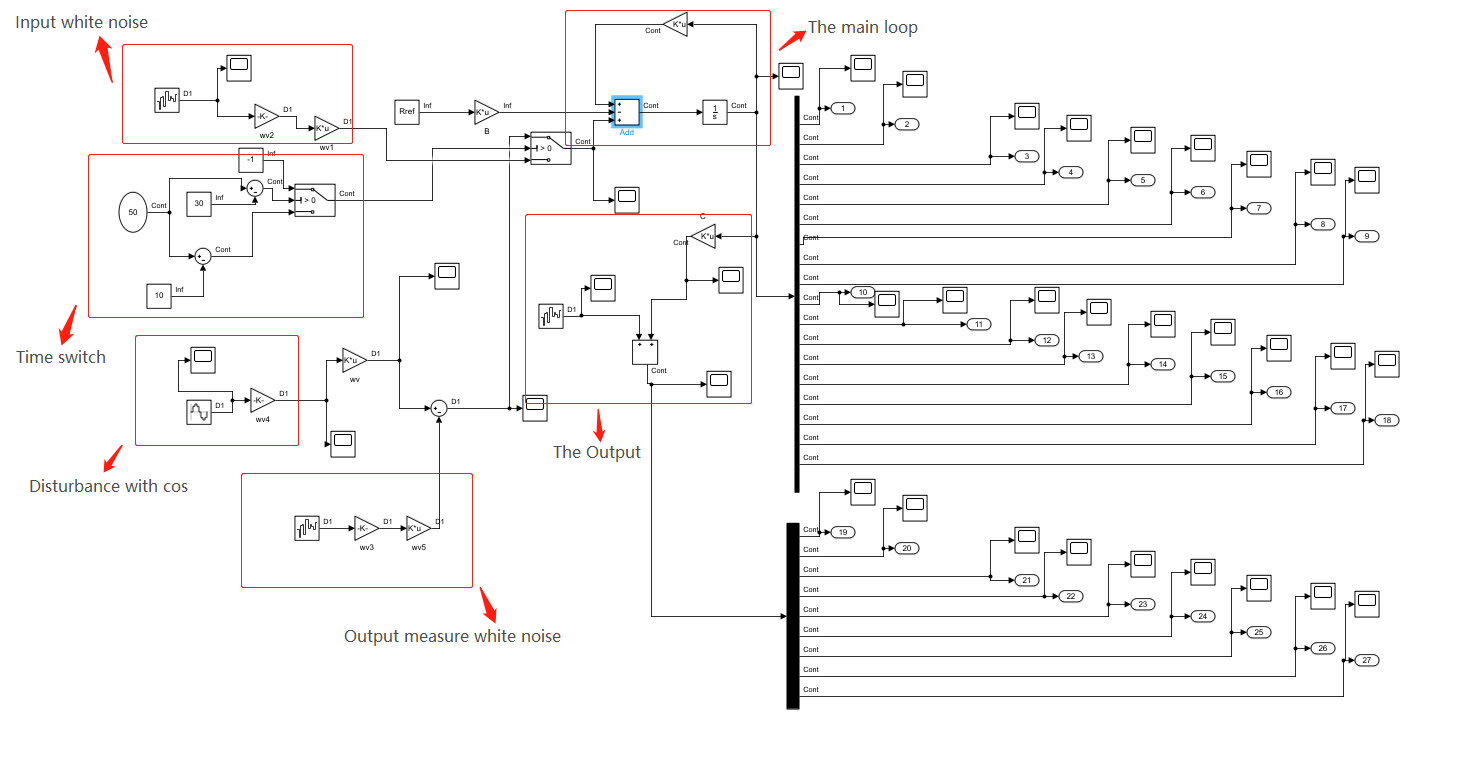
\includegraphics[width=20cm,height=10cm,scale=0.6]{block_diagram.png}
    \caption{The Unmanned Helicopter LQG Controller diagram}
    \label{fig:label}
    \end{figure}

Then,I will show the state and error,and y output from figure 2 and figure 3:\\
\begin{figure}[H]
    \centering
    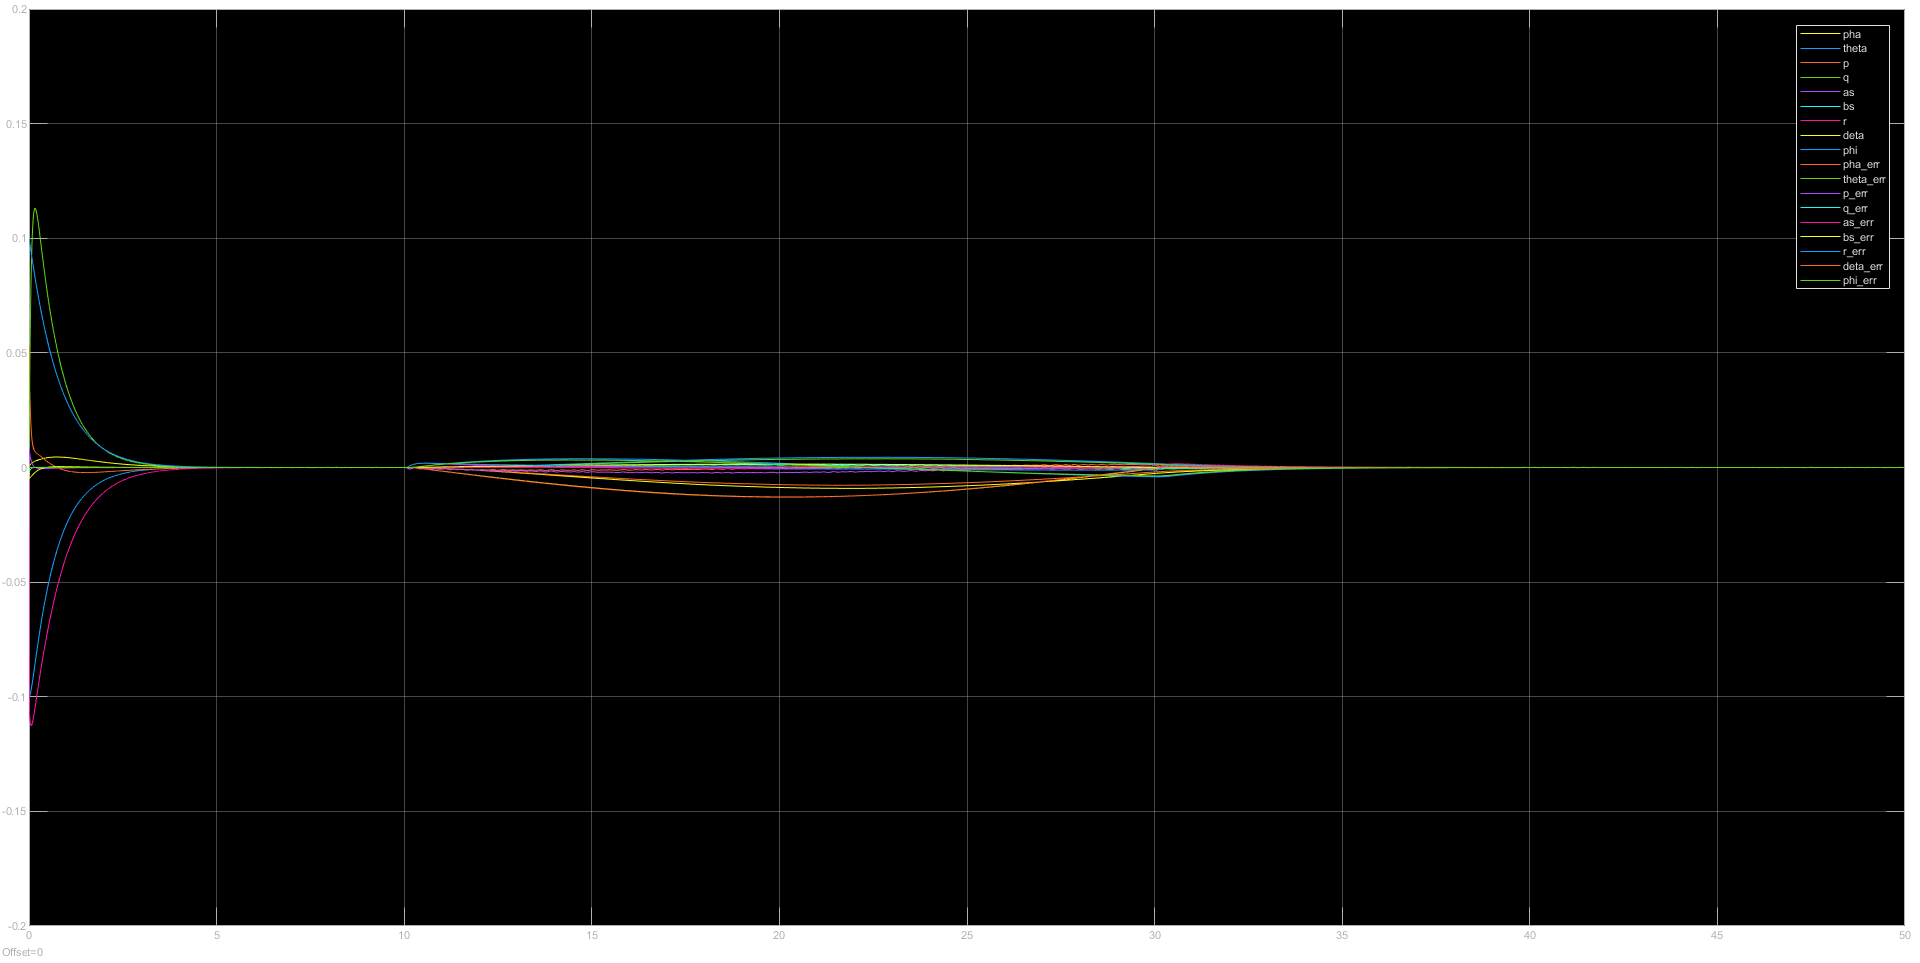
\includegraphics[width=20cm,height=10cm,scale=0.6]{state_18.png}
    \caption{The Plant state x and error}
    \label{fig:label}
    \end{figure}

\begin{figure}[H]
    \centering
    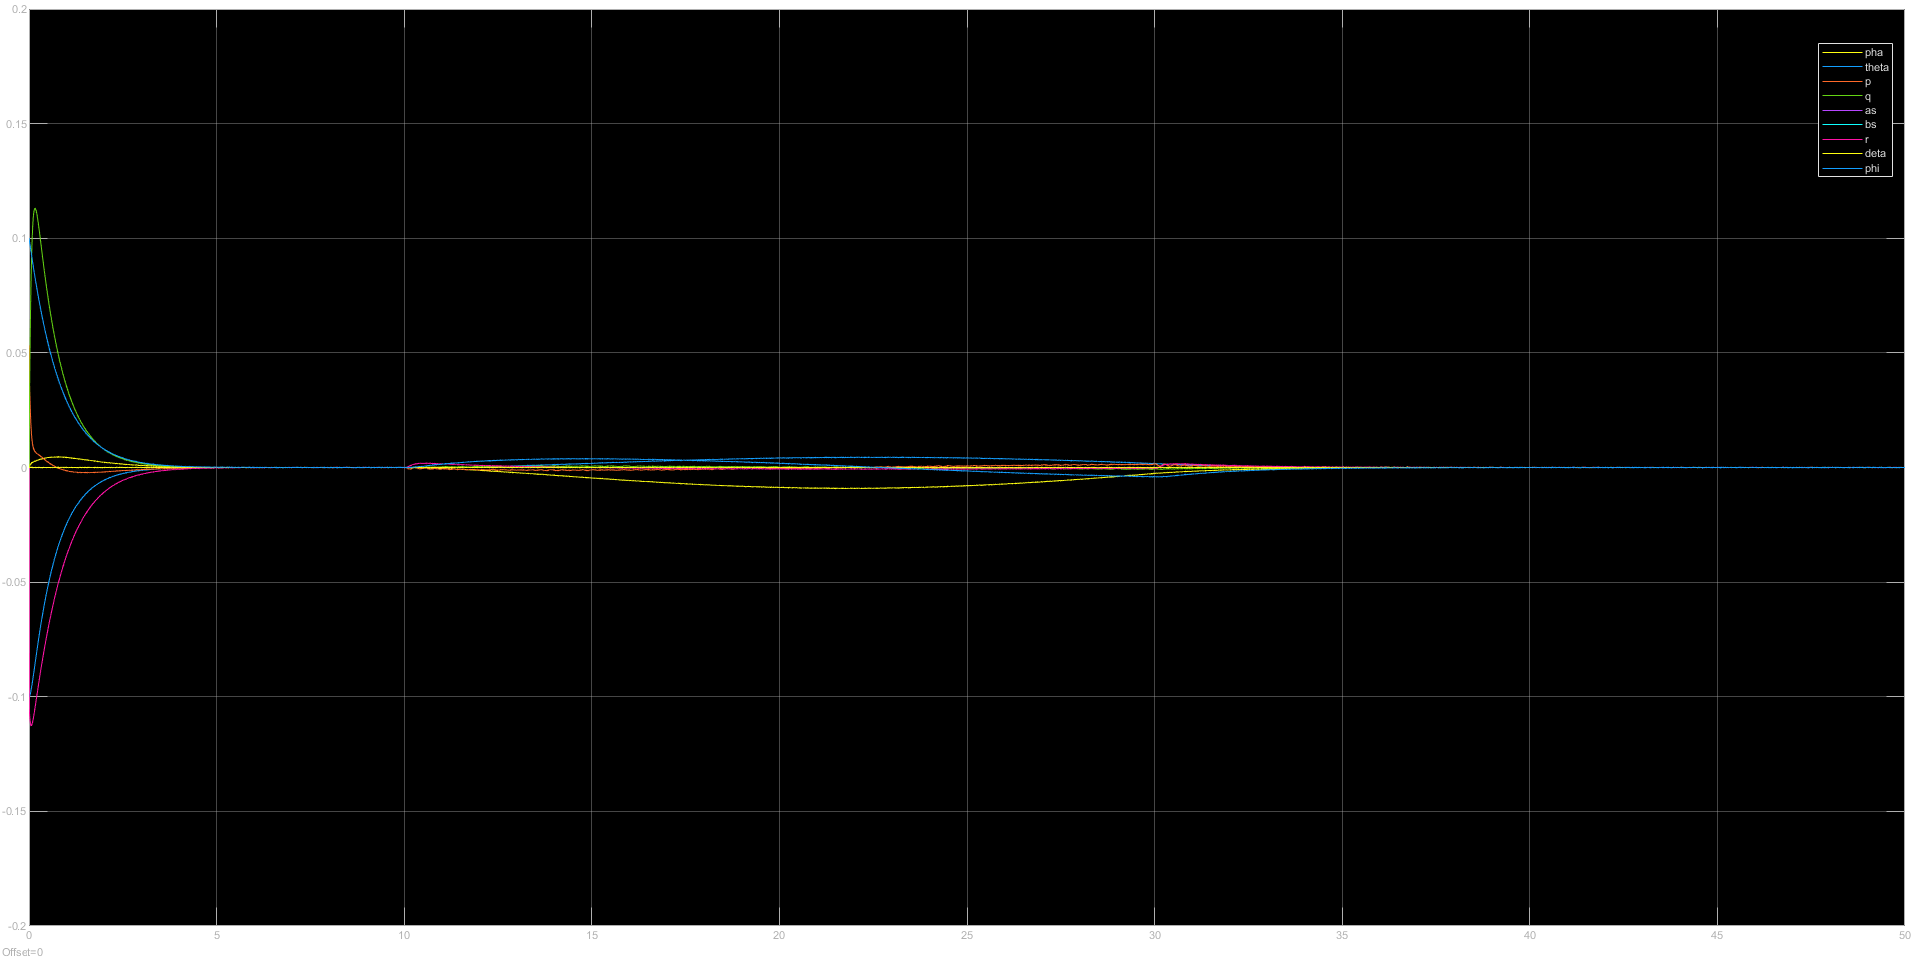
\includegraphics[width=20cm,height=10cm,scale=0.6]{state_output.png}
    \caption{The Plant y output}
    \label{fig:label}
    \end{figure}
At last,I will show all state and output respectively.\\
\begin{figure}[H]
        \centering
        \subfloat[State:pha]{{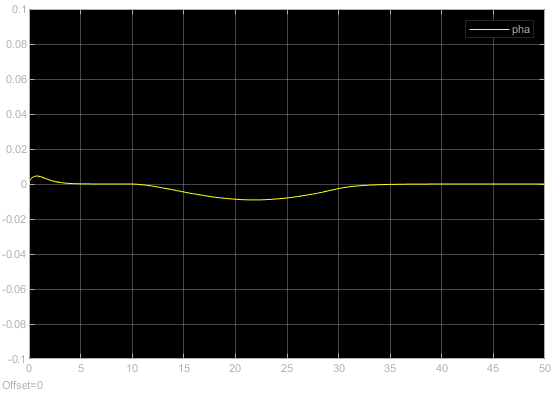
\includegraphics[width=8cm,height=8cm]{pha.png} }}%
        \qquad
        \subfloat[Error:pha]{{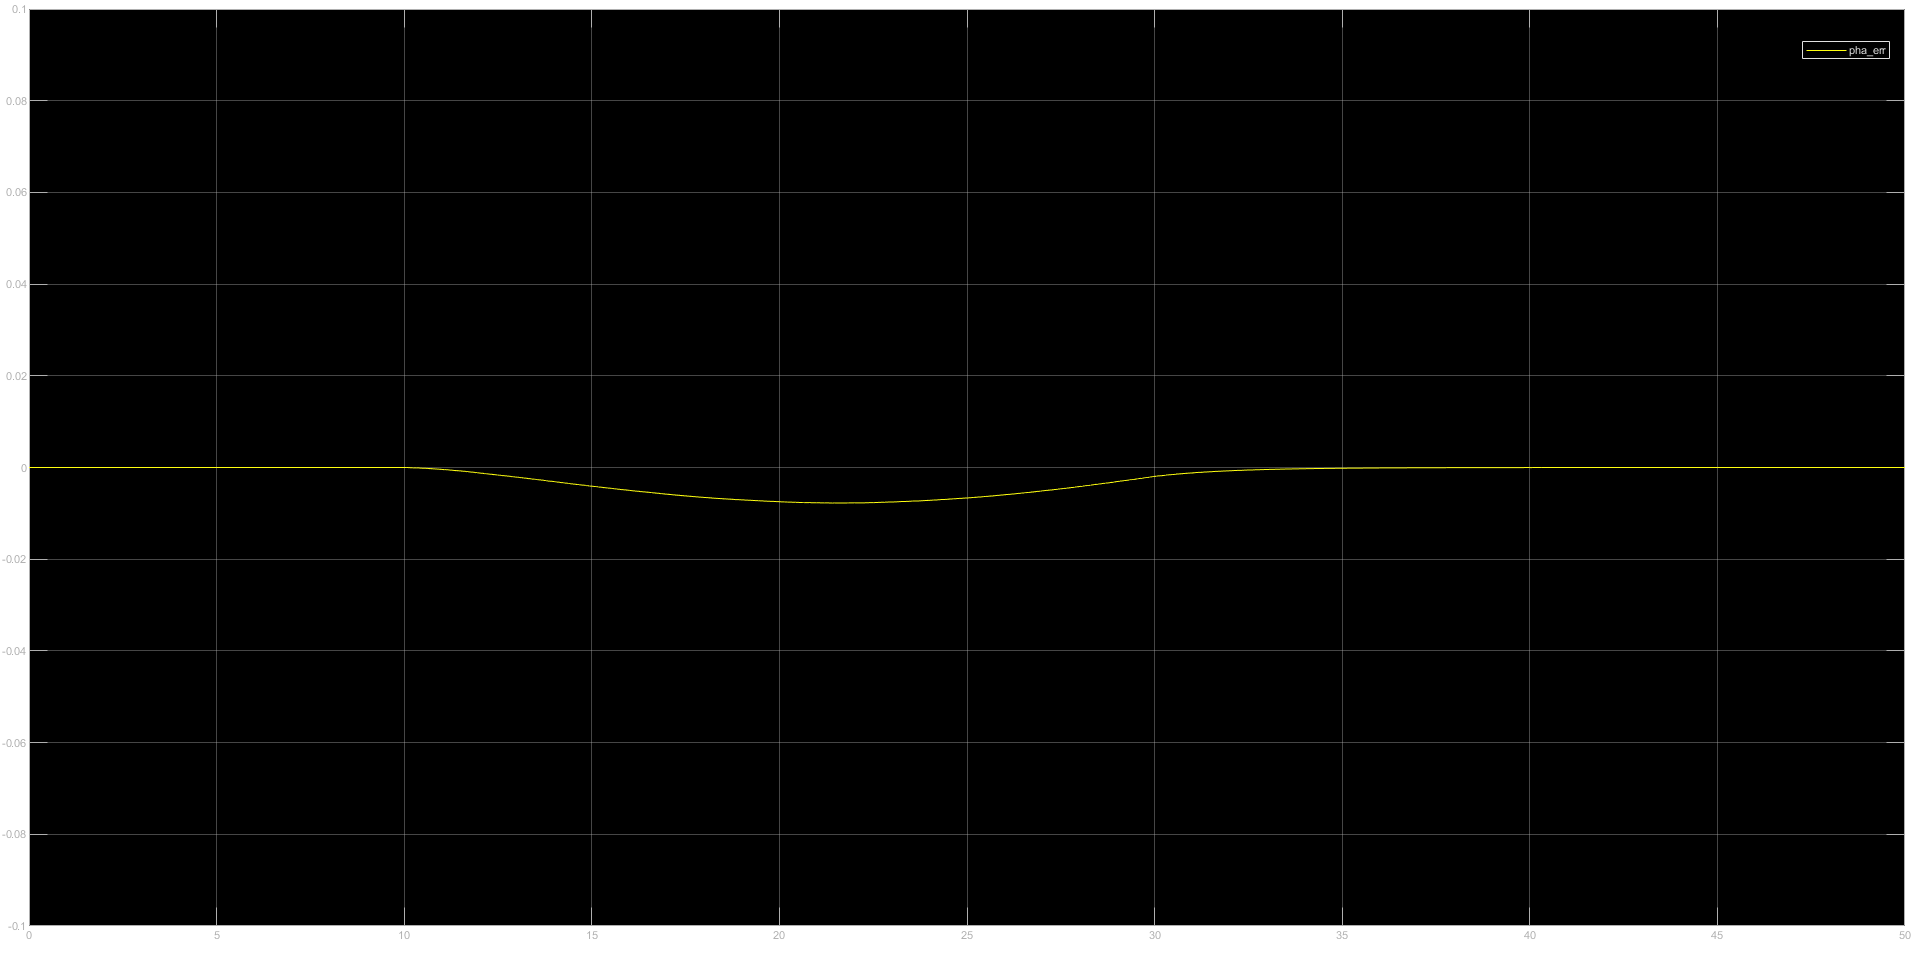
\includegraphics[width=7.9cm,height=7.9cm]{pha_err.png} }}%
        \caption{Pha state and error}
        \label{fig:example}%
    \end{figure}

\begin{figure}[H]
    \centering
    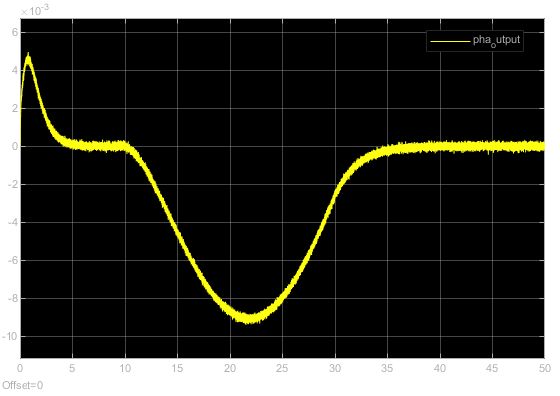
\includegraphics[width=8cm,height=8cm,scale=0.6]{pha_output.png}
    \caption{The Plant Pha output}
    \label{fig:label}
    \end{figure}
\begin{figure}[H]
        \centering
        \subfloat[State:Theta]{{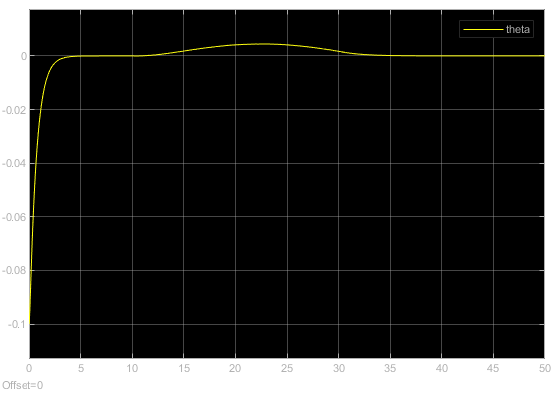
\includegraphics[width=8cm,height=8cm]{theta.png} }}%
        \qquad
        \subfloat[Error:Theta]{{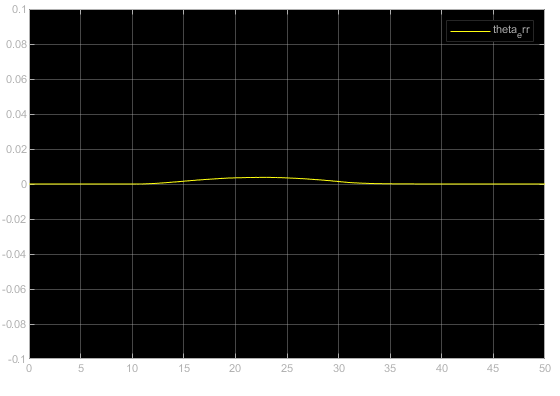
\includegraphics[width=7.9cm,height=7.9cm]{theta_err.png} }}%
        \caption{Pha state and error}
        \label{fig:example}%
    \end{figure}
\begin{figure}[H]
    \centering
    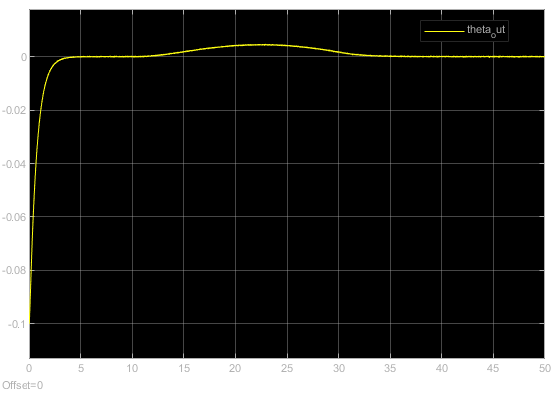
\includegraphics[width=8cm,height=8cm,scale=0.6]{theta_out.png}
    \caption{The Plant Theta output}
    \label{fig:label}
    \end{figure}

\begin{figure}[H]
        \centering
        \subfloat[State:p]{{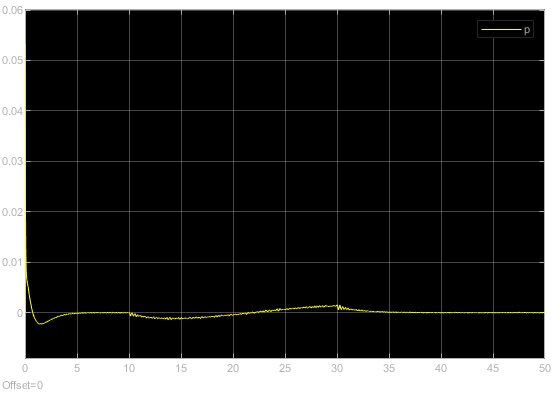
\includegraphics[width=8cm,height=8cm]{p.png} }}%
        \qquad
        \subfloat[Error:p]{{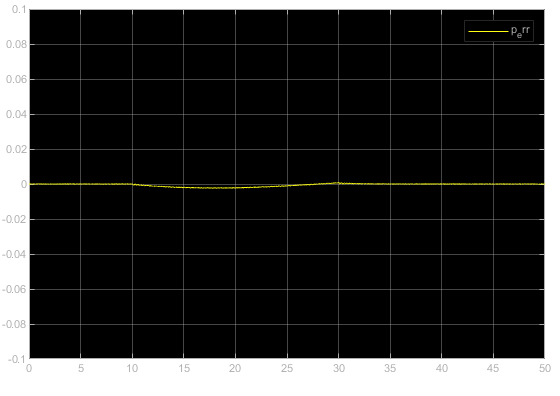
\includegraphics[width=7.9cm,height=7.9cm]{p_err.png} }}%
        \caption{p state and error}
        \label{fig:example}%
    \end{figure}
\begin{figure}[H]
    \centering
    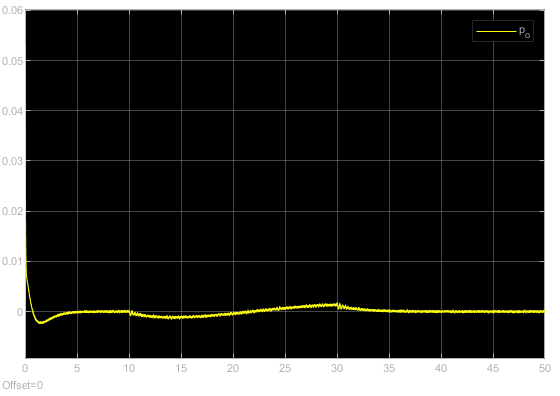
\includegraphics[width=8cm,height=8cm,scale=0.6]{p_o.png}
    \caption{The Plant p output}
    \label{fig:label}
    \end{figure}
\begin{figure}[H]
        \centering
        \subfloat[State:q]{{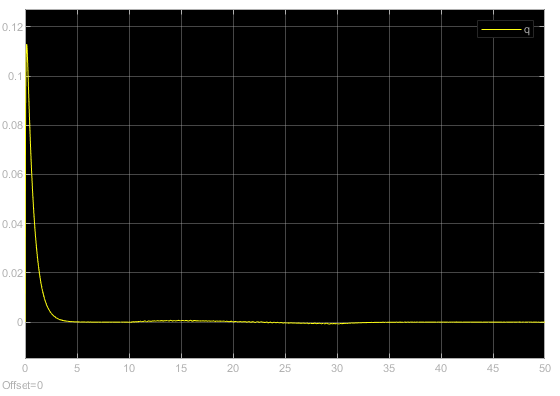
\includegraphics[width=8cm,height=8cm]{q.png} }}%
        \qquad
        \subfloat[Error:q]{{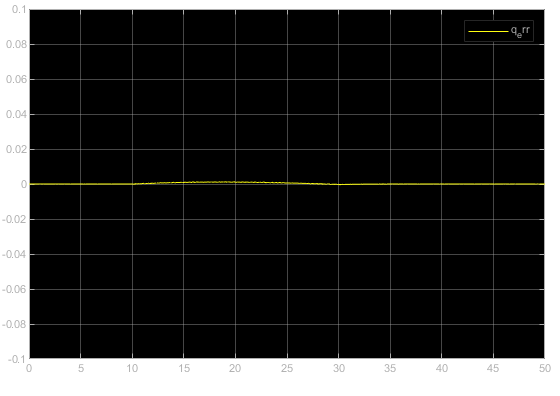
\includegraphics[width=7.9cm,height=7.9cm]{q_err.png} }}%
        \caption{q state and error}
        \label{fig:example}%
    \end{figure}
\begin{figure}[H]
    \centering
    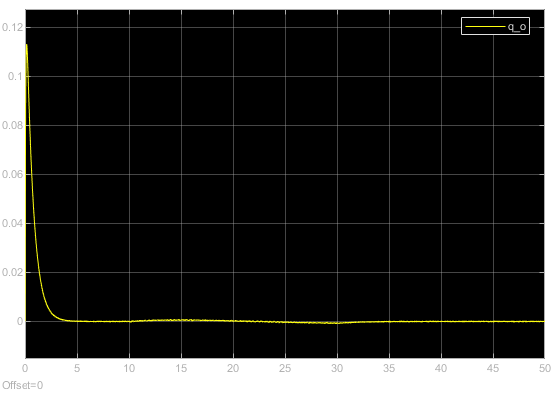
\includegraphics[width=8cm,height=8cm,scale=0.6]{q_o.png}
    \caption{The Plant q output}
    \label{fig:label}
    \end{figure}
    \begin{figure}[H]
        \centering
        \subfloat[State:as]{{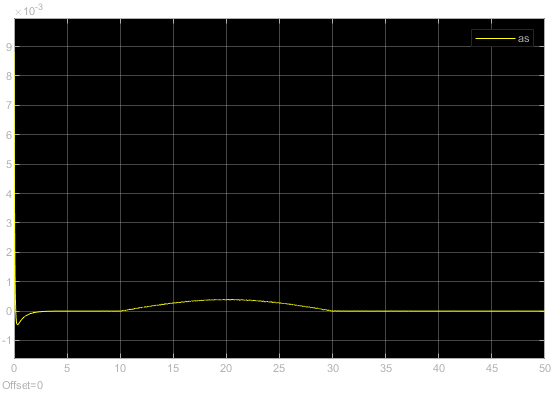
\includegraphics[width=8cm,height=8cm]{as.png} }}%
        \qquad
        \subfloat[Error:as]{{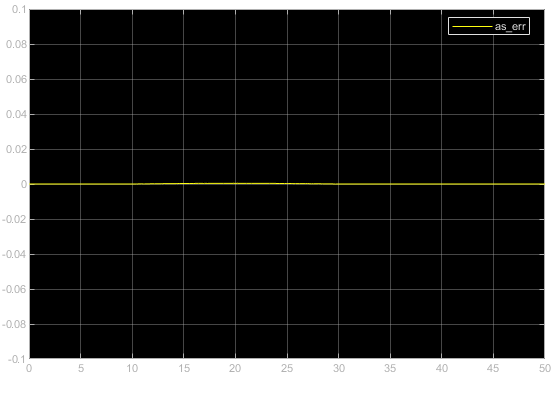
\includegraphics[width=7.9cm,height=7.9cm]{as_err.png} }}%
        \caption{as state and error}
        \label{fig:example}%
    \end{figure}
\begin{figure}[H]
    \centering
    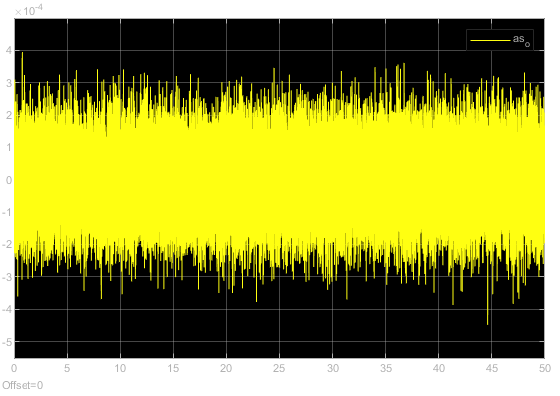
\includegraphics[width=8cm,height=8cm,scale=0.6]{as_o.png}
    \caption{The Plant as output}
    \label{fig:label}
    \end{figure}
\begin{figure}[H]
        \centering
        \subfloat[State:bs]{{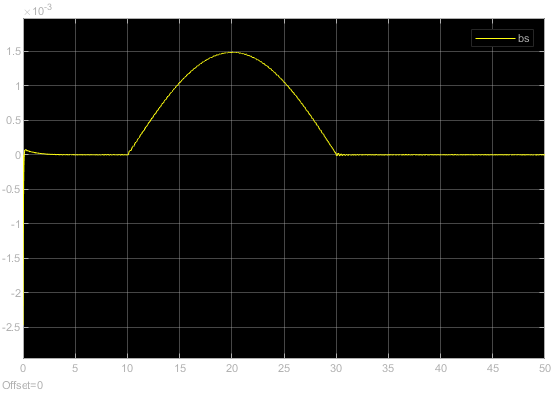
\includegraphics[width=8cm,height=8cm]{bs.png} }}%
        \qquad
        \subfloat[Error:bs]{{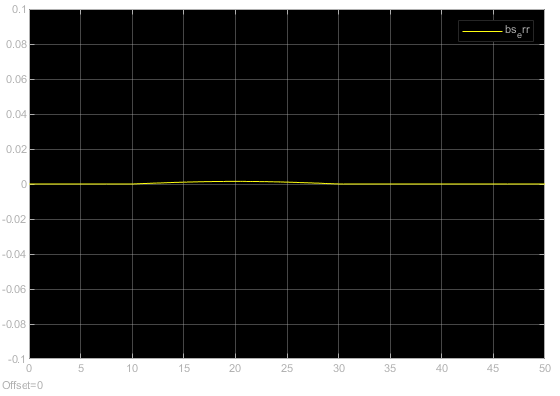
\includegraphics[width=7.9cm,height=7.9cm]{bs_err.png} }}%
        \caption{bs state and error}
        \label{fig:example}%
    \end{figure}
\begin{figure}[H]
    \centering
    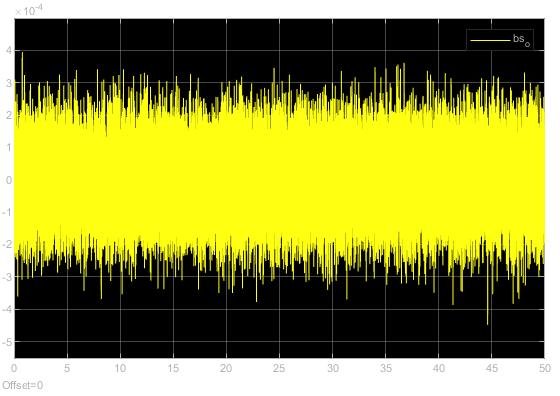
\includegraphics[width=8cm,height=8cm,scale=0.6]{bs_o.png}
    \caption{The Plant bs output}
    \label{fig:label}
    \end{figure}    
    \begin{figure}[H]
        \centering
        \subfloat[State:r]{{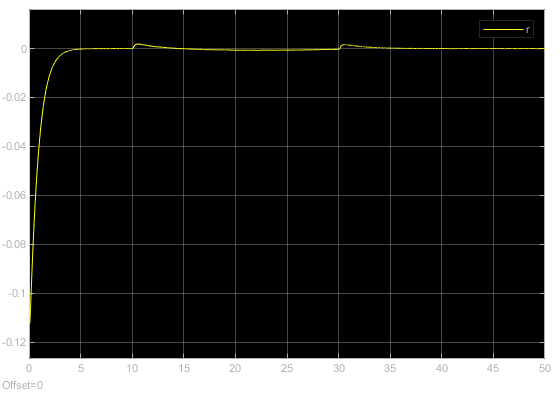
\includegraphics[width=8cm,height=8cm]{r.png} }}%
        \qquad
        \subfloat[Error:r]{{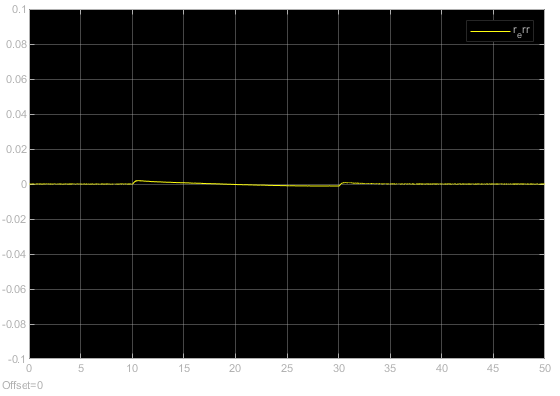
\includegraphics[width=7.9cm,height=7.9cm]{r_err.png} }}%
        \caption{r state and error}
        \label{fig:example}%
    \end{figure}
\begin{figure}[H]
    \centering
    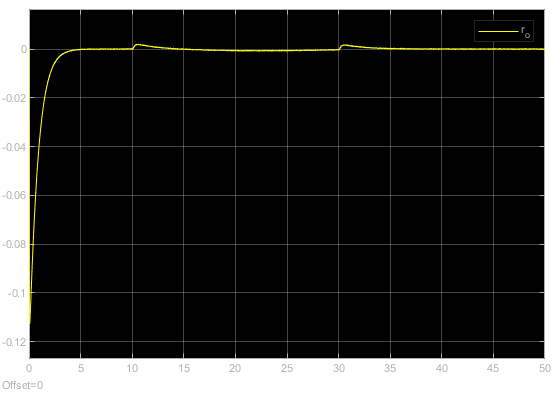
\includegraphics[width=8cm,height=8cm,scale=0.6]{r_o.png}
    \caption{The Plant r output}
    \label{fig:label}
    \end{figure}
    \begin{figure}[H]
        \centering
        \subfloat[State:deta]{{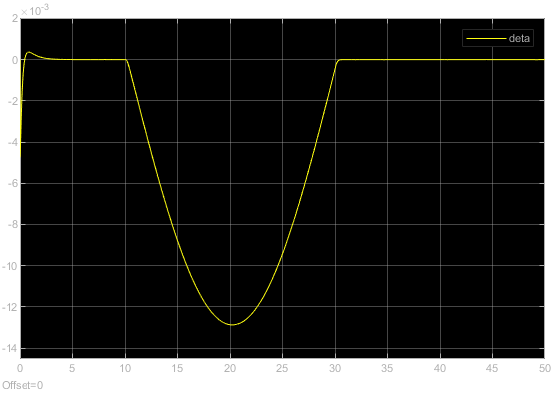
\includegraphics[width=8cm,height=8cm]{deta.png} }}%
        \qquad
        \subfloat[Error:deta]{{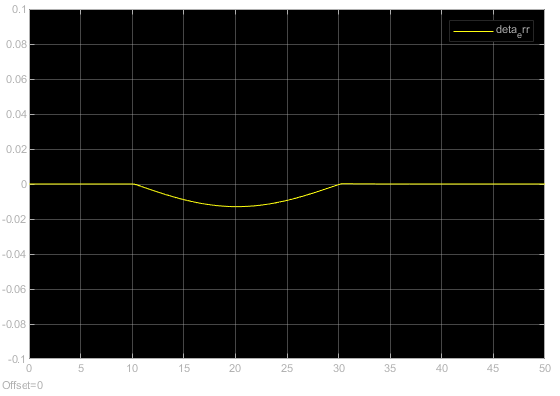
\includegraphics[width=7.9cm,height=7.9cm]{deta_err.png} }}%
        \caption{deta state and error}
        \label{fig:example}%
    \end{figure}
\begin{figure}[H]
    \centering
    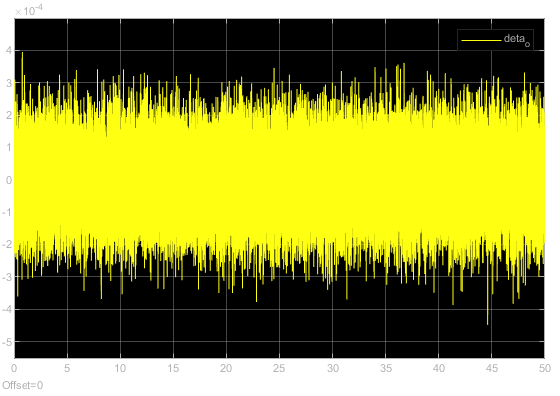
\includegraphics[width=8cm,height=8cm,scale=0.6]{deta_o.png}
    \caption{The Plant deta output}
    \label{fig:label}
    \end{figure}
\begin{figure}[H]
        \centering
        \subfloat[State:phi]{{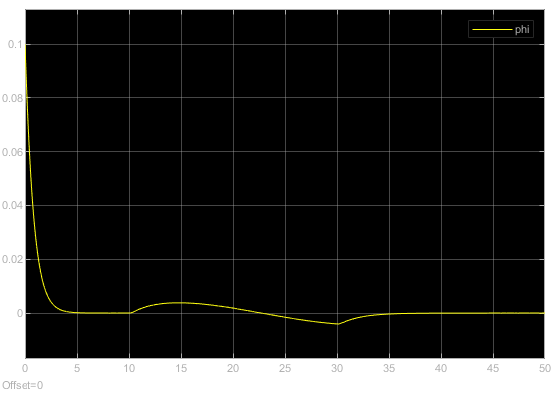
\includegraphics[width=8cm,height=8cm]{phi.png} }}%
        \qquad
        \subfloat[Error:phi]{{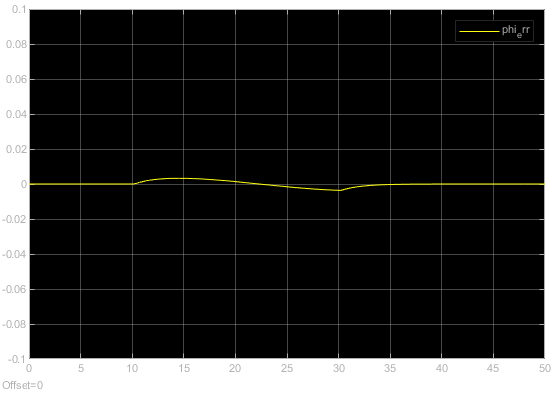
\includegraphics[width=7.9cm,height=7.9cm]{phi_err.png} }}%
        \caption{phi state and error}
        \label{fig:example}%
    \end{figure}
\begin{figure}[H]
    \centering
    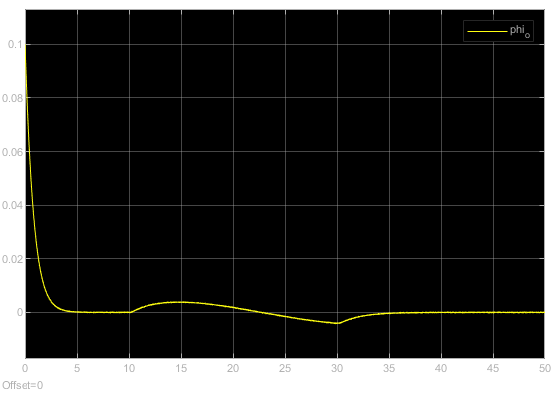
\includegraphics[width=8cm,height=8cm,scale=0.6]{phi_o.png}
    \caption{The Plant phi output}
    \label{fig:label}
    \end{figure}     

\end{enumerate}
\begin{thebibliography}{00}
    \bibitem{b1} Liu X , Chen B M , Lin Z . Linear systems toolkit in Matlab: structural decompositions and their applications[J]. Journal of Control Theory and Applications, 2005, 3(3):p.287-294.
    \bibitem{b2} C. T. Chen, Linear System Theory and Design, Holt, Rinehart $&$ Winston, 1984
    \bibitem{b3} B. M. Chen, Robust and $H\infty$ Control, Springer, 2000
    \bibitem{b4} G. Cai, B. M. Chen, T. H. Lee, Unmanned Rotorcraft Systems, Springer, 2011
\end{thebibliography}
\end{document}